% TODO skratiti arhitekturu

\begin{frame}{CEGIS}
    \begin{itemize}
		\item Ideja:
			\begin{itemize}
				\item Definiše se specifikacija programa u vidu formule
		    	\item SMT rešavač pronalazi program koji zadovoljava specifikaciju
			\end{itemize}    	
    	\item Problem: previše ulaza 
        \item \emph{Koji je najmanji podskup ulaza koji je potrebno razmatrati da bi se sintetisao program koji zadovoljava date specifikacije?}
        \item CEGIS pokušava da reši ovaj problem
        \item Iterativno se povećava prostor pretrage i pronalazi program kandidat za rešenje
        \item Drugi SMT rešavač pronalazi kontraprimer za nađeni kandidat
		\item Ako ne postoji kontraprimer, kandidat je traženi program
    \end{itemize}
\end{frame}

\begin{frame}[fragile]{CEGIS - Arhitektura}
    \begin{itemize}
    	\item Pretraga vođena kontraprimerima \\(eng. \emph{Counterexample-Guided Inductive Synthesis})
        \item Dve faze: 
        	\begin{itemize}
        		\item \emph{Faza sinteze} - pronalazi program kandidat
        		\item \emph{Faza verifikacije} - proverava da li kandidat zadovoljava specifikaciju 
        	\end{itemize}
    \end{itemize}
    \begin{figure}
        \begin{center}
            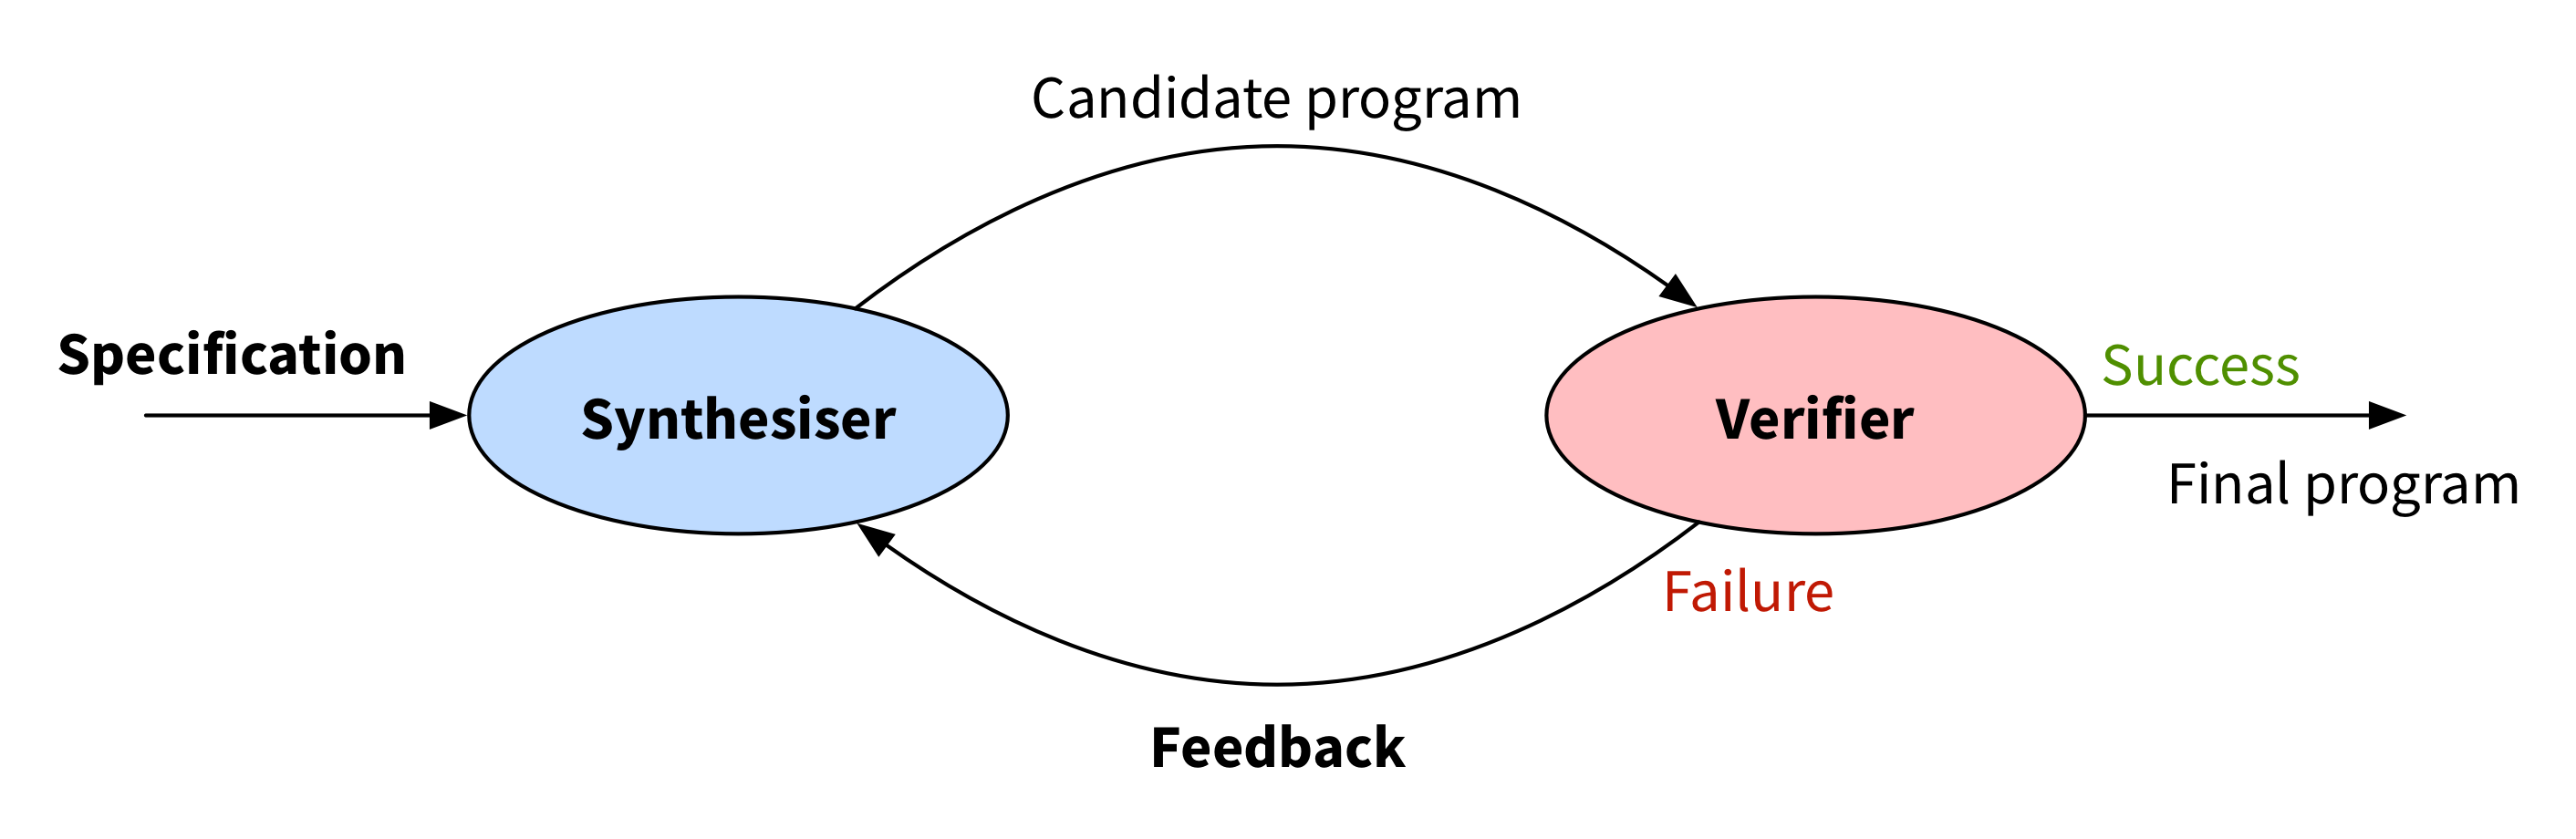
\includegraphics[scale=0.4]{../resources/cegis.png}
        \end{center}
        \caption{CEGIS petlja}
    \end{figure}
\end{frame}

\begin{frame}{CEGIS}
    \begin{itemize}
        \item Da bismo u potpunosti definisali CEGIS sintezu programa, potrebno je odgovoriti na sledeća pitanja:
        \begin{itemize}
            \item Kako treba da izgleda specifikacija traženog programa?
            \item Kako ćemo vršiti sintezu programa kandidata?
            \item Kako da proverimo da li program kandidat zadovoljava specifikacije?
            \item Kako da prosledimo povratne informacije za buduće kandidate?
        \end{itemize}
    \end{itemize}
\end{frame}
